\chapter{AWS Docker Deployment}
\ChapterLabel{AWSDockerDeployment}
\index{AWS}
\index{EC2}
\index{Docker!cloud deployment}

\section{Overview}
\begin{devopsNote}[Deviation from the assignment, disclosed]
This assignment's instructions ask for a \textbf{Digital Ocean Droplet}
running Docker. Group~1 deployed to an \textbf{AWS EC2 instance} instead,
performing the exact same role: one cloud virtual machine running Docker and
serving the website. This substitution is a group choice, not something the
assignment itself offered for this item; it is made because the semester
project (\ChapterRef{ProjectProposal}) is built on AWS, and standing up the
account, IAM users, budget alert, and security-group model here means that
work is reused rather than duplicated on a second cloud provider the group
would not otherwise use. Table~\ref{Table:DOtoAWS} maps every Digital Ocean
concept the assignment describes onto its AWS equivalent, so the deployment
can be read and graded as a direct substitute. If a literal Digital Ocean
Droplet is required, the group will redeploy there using \texttt{doctl} in
place of the AWS CLI; the Docker image and application are unchanged either
way.
\end{devopsNote}
The cloud server is an \gls{ec2} instance, which plays the role of a Droplet.
It runs the two-button website from \ChapterRef{ClassBasedWebsite} in a
Docker container and serves it on port~80.

\begin{devopsNote}[Live website]
\textbf{Website:} \texttt{\WebsiteURL}\\
\textbf{Health check:} \texttt{\WebsiteURL/health}\\
\textbf{Source:} \url{\RepoURL}\\[3pt]
\small The address is set by the \texttt{\string\WebsiteURL} macro in
\texttt{devopsAssignment.tex}. Replace the placeholder with the public DNS name
printed by \texttt{launch-ec2.sh} (Section~\ref{Section:AWSCLI}).
\end{devopsNote}

\section{Digital Ocean to AWS Mapping}
\begin{tabularx}{\linewidth}{L{3.6cm}L{4.4cm}Y}
\caption{Digital Ocean Concepts and Their AWS Equivalents\label{Table:DOtoAWS}}\\
\toprule \textbf{Digital Ocean} & \textbf{AWS} & \textbf{Used here}\\ \midrule
\endfirsthead
\toprule \textbf{Digital Ocean} & \textbf{AWS} & \textbf{Used here}\\ \midrule
\endhead \bottomrule \endlastfoot
Droplet & \gls{ec2} instance & \texttt{t3.micro}, Free Tier eligible\\
Droplet image (Ubuntu) & \gls{ami} & Amazon Linux 2023\\
Cloud Firewall & \gls{securitygroup} & HTTP 80 and HTTPS 443 open; SSH 22 from one IP\\
SSH key & EC2 key pair & \texttt{ssw590-group1-key}\\
Cloud-init user data & EC2 \gls{userdata} & \texttt{deploy/aws/ec2-user-data.sh}\\
\texttt{doctl} CLI & AWS CLI v2 & \texttt{deploy/aws/launch-ec2.sh}\\
Docker 1-Click Droplet & Docker installed by \texttt{dnf} & Docker from the AL2023 repository\\
\end{tabularx}

\section{Prerequisites and Account Security}
\begin{enumerate}
\item Create an AWS account and enable multi-factor authentication on the root
user. Do not use the root user for daily work.
\item In IAM, create a user for each member with console access and the
\texttt{AmazonEC2FullAccess} policy (or a narrower custom policy), and create an
access key for CLI use. Keys are stored only in \texttt{\textasciitilde/.aws/credentials}
on the member's machine and are never committed.
\item In Billing, create a monthly budget (for example \$5) with an e-mail
alert so a forgotten instance is noticed quickly.
\item Install and configure the AWS CLI v2:
\end{enumerate}
\begin{minted}{bash}
brew install awscli                # macOS; see AWS docs for Windows/Linux
aws configure                      # access key, secret, region us-east-1, output json
aws sts get-caller-identity        # confirms the CLI is signed in as the IAM user
\end{minted}

\section{Deployment Steps}
Two equivalent paths are documented: the AWS Console (closest to creating a
Droplet in the Digital Ocean web UI) and a scripted CLI path that the group uses
for repeatable deployments. Both run the same \gls{userdata} script.

\subsection{The Bootstrap Script}
\label{Section:Bootstrap}
At first boot the instance runs this script as root. It installs Docker and Git,
clones the group repository, builds the image, and starts the container with a
restart policy so the site comes back after a reboot. Port~80 on the host is
mapped to port~3000 inside the container.
\inputminted{bash}{../deploy/aws/ec2-user-data.sh}

\subsection{Private Repository and the Deploy Key}
\label{Section:DeployKey}
\begin{devopsNote}[What actually happened on this deployment]
The group repository is \textbf{private}. The bootstrap script in
Section~\ref{Section:Bootstrap} clones it anonymously over HTTPS, which works
only for a public repository. On the real run, cloud-init's \gls{userdata}
step failed with \texttt{fatal: could not read Username for
`https://github.com': No such device or address}, so the container never
started automatically. This was diagnosed from the instance's console output
(\texttt{aws ec2 get-console-output}) rather than guessed.

The fix was to generate an \texttt{ed25519} key pair on the instance, add its
\emph{public} half as a read-only \textbf{deploy key} on the GitHub repository
(Settings $\rightarrow$ Deploy keys), and then run the same clone, build, and
run commands shown in Section~\ref{Section:ManualCommands} by hand over SSH,
using \texttt{git@github.com:\dots} instead of the HTTPS URL. The private key
never leaves the instance; the deploy key is read-only and scoped to this one
repository. A future improvement would be to bake the deploy key into the AMI
or pass it through \gls{userdata} (e.g.\ via AWS Secrets Manager) so first
boot succeeds without a manual step; that is not yet done.
\end{devopsNote}

\subsection{Path A: AWS Console}
\begin{enumerate}
\item Open \textbf{EC2 $\rightarrow$ Launch instance}. Name it
\texttt{ssw590-group1-web}.
\item Choose the \textbf{Amazon Linux 2023} \gls{ami} (64-bit x86) and instance
type \textbf{t3.micro}.
\item Under \textbf{Key pair}, create \texttt{ssw590-group1-key} (RSA,
\texttt{.pem}) and save the downloaded file to \texttt{\textasciitilde/.ssh/}.
\item Under \textbf{Network settings}, create a security group that allows
\textbf{SSH} from \emph{My IP} and \textbf{HTTP} from \emph{Anywhere}.
\item Expand \textbf{Advanced details}. In the \textbf{User data} box, paste
the contents of \path{deploy/aws/ec2-user-data.sh}.
\item Click \textbf{Launch instance}, wait for \emph{2/2 status checks passed},
and copy the \textbf{Public IPv4 DNS} from the instance page.
\end{enumerate}

\subsection{Path B: AWS CLI}
\label{Section:AWSCLI}
The launch script creates the key pair and security group if they do not exist,
looks up the latest Amazon Linux 2023 \gls{ami} from AWS's public SSM parameter,
launches the instance with the bootstrap script, and prints the website address.
\inputminted{bash}{../deploy/aws/launch-ec2.sh}
It is run from the repository root:
\begin{minted}{bash}
git clone https://github.com/brahmi9811/ssw-590-group1.git
cd ssw-590-group1
./deploy/aws/launch-ec2.sh
\end{minted}

\subsection{Manual Commands on the Instance}
\label{Section:ManualCommands}
For transparency, these are the same steps the bootstrap script automates,
typed by hand after connecting over SSH. They are also the steps to follow if
the user data is omitted.
\begin{minted}{bash}
chmod 400 ~/.ssh/ssw590-group1-key.pem
ssh -i ~/.ssh/ssw590-group1-key.pem ec2-user@<EC2-PUBLIC-DNS>

# on the instance
sudo dnf update -y
sudo dnf install -y docker git
sudo systemctl enable --now docker
sudo usermod -aG docker ec2-user && newgrp docker
docker --version

git clone https://github.com/brahmi9811/ssw-590-group1.git
cd ssw-590-group1/website/color-buttons-app
docker build -t color-buttons-app:2.0 .
docker run -d --name color-buttons-app --restart unless-stopped \
  -p 80:3000 color-buttons-app:2.0
docker ps
\end{minted}

\section{Verification}
\subsection{Pre-deployment Check on a Workstation}
Before deploying, the exact image that the instance builds was built and run on
a group member's workstation (Docker 29.4.2, Apple silicon), published on host
port~8081. The output below is from that real run.
\inputminted{console}{../evidence/local-build-run.txt}
\inputminted{console}{../evidence/local-checks.txt}
The page was then opened in a browser; clicking \emph{Red} and then \emph{Blue}
changed the page background to red and then blue, served by the class-based
code in \ChapterRef{ClassBasedWebsite}.

\subsection{Cloud Verification}
After launch, the following commands confirm the deployment from any machine.
Paste their output into \path{evidence/aws-checks.txt} and save a browser
screenshot as \path{evidence/aws-website.png}.
\begin{minted}{bash}
curl -s http://<EC2-PUBLIC-DNS>/health        # {"status":"ok",...}
curl -sI http://<EC2-PUBLIC-DNS>/ | head -1   # HTTP/1.1 200 OK
ssh -i ~/.ssh/ssw590-group1-key.pem ec2-user@<EC2-PUBLIC-DNS> \
  'docker ps --format "{{.Names}} {{.Status}} {{.Ports}}"'
\end{minted}
\inputminted{console}{../evidence/aws-checks.txt}

\begin{devopsNote}[A browser-only problem, and why port 443 is also open]
\texttt{curl} reached the site over plain HTTP the whole time, but a browser
pointed at the same \texttt{http://} address showed
\texttt{ERR\_CONNECTION\_TIMED\_OUT}. The cause was not the server: current
Chrome and mobile browsers silently upgrade \texttt{http://} requests on
\texttt{amazonaws.com} hosts to \texttt{https://} (an HSTS/HTTPS-first
behavior that is hard-coded for many cloud domains and is not something a
per-site browser setting can turn off), so the browser was actually trying
port~443, which the security group did not yet open. The fix was to open
port~443 (Table~\ref{Table:DOtoAWS}'s security group) and put
\texttt{nginx} in front of the container as a TLS-terminating reverse proxy
on port~443, forwarding to the existing app on port~80. The connection now
succeeds for any browser on any network. Figure~\ref{Figure:AWSWebsite}
shows the deployed site in a browser, including the two-button click
behavior working against the live cloud instance.
\end{devopsNote}

\begin{figure}[htbp]
\centering
\fbox{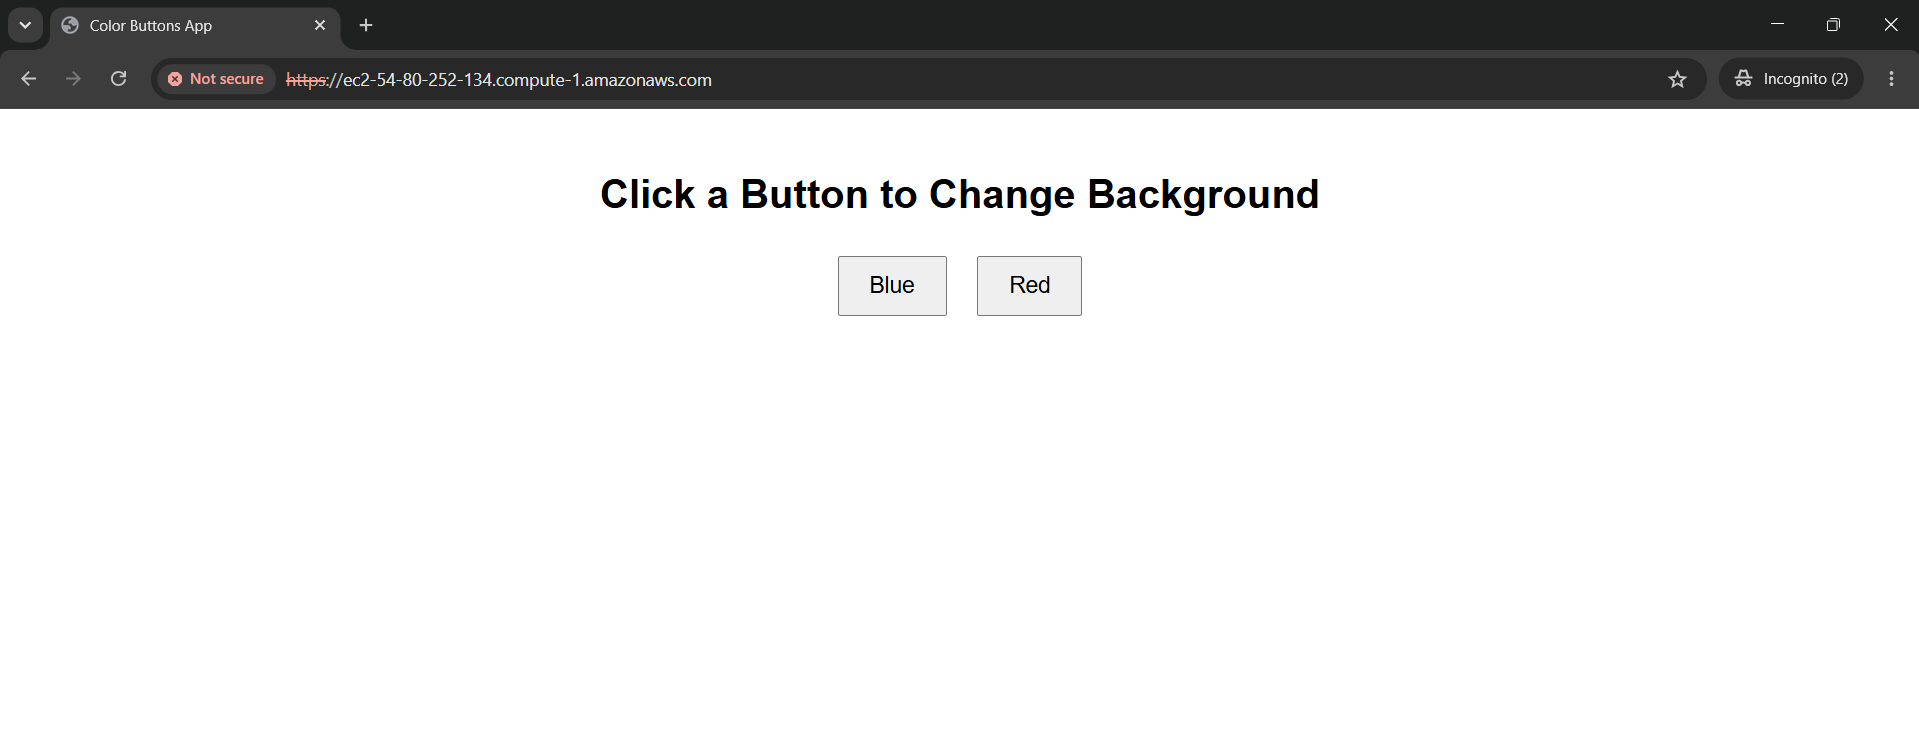
\includegraphics[width=0.7\linewidth]{../evidence/aws-website.png}}
\caption{The deployed site at the public EC2 address, on load.}
\label{Figure:AWSWebsite}
\end{figure}

\begin{figure}[htbp]
\centering
\fbox{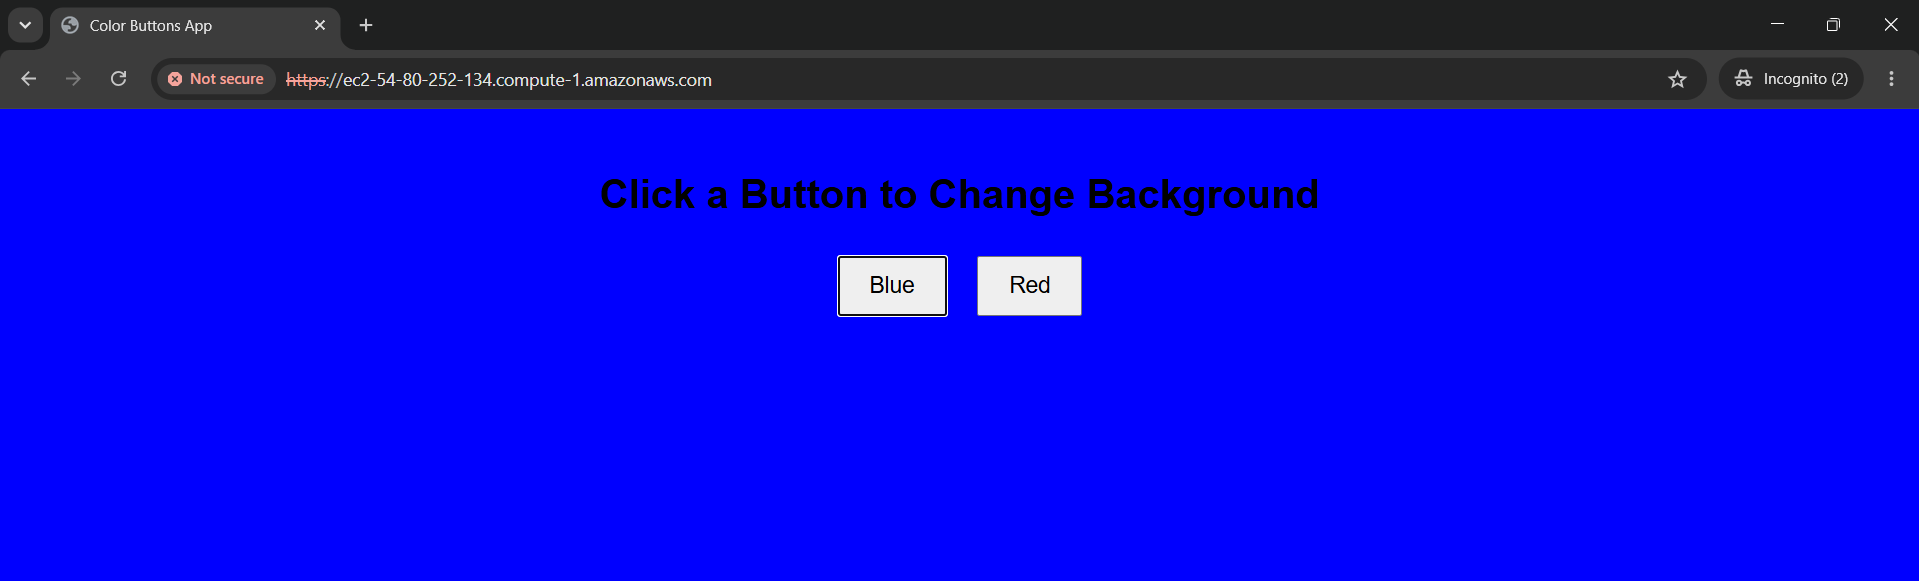
\includegraphics[width=0.7\linewidth]{../evidence/aws-website-blue.png}}
\caption{The same deployment after clicking \emph{Blue}.}
\label{Figure:AWSWebsiteBlue}
\end{figure}

\begin{figure}[htbp]
\centering
\fbox{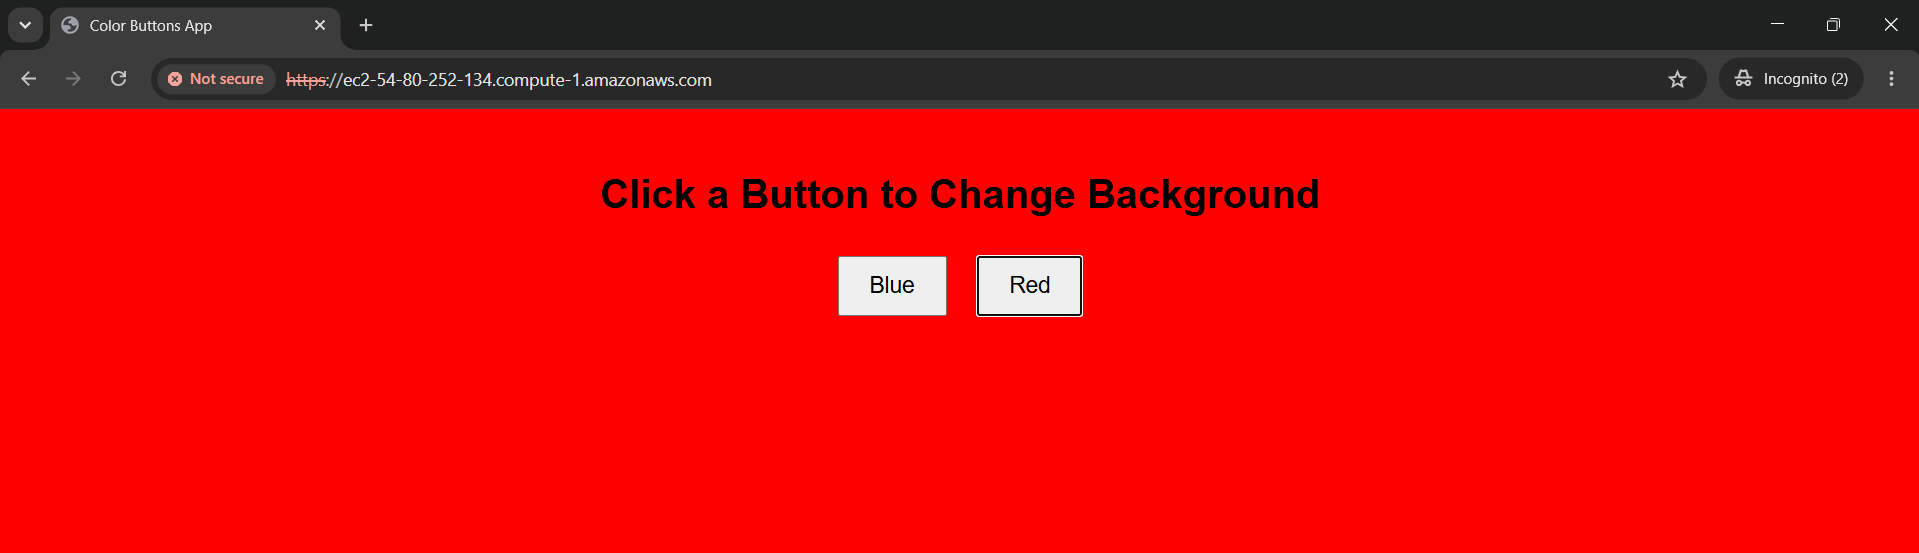
\includegraphics[width=0.7\linewidth]{../evidence/aws-website-red.png}}
\caption{The same deployment after clicking \emph{Red}. Together with
Figures~\ref{Figure:AWSWebsite} and~\ref{Figure:AWSWebsiteBlue}, this
confirms the class-based code from \ChapterRef{ClassBasedWebsite} runs
correctly on the real cloud deployment, not just locally.}
\label{Figure:AWSWebsiteRed}
\end{figure}

\begin{tabularx}{\linewidth}{L{5.2cm}L{2.2cm}Y}
\caption{Deployment Checklist\label{Table:AWSChecklist}}\\
\toprule \textbf{Check} & \textbf{Status} & \textbf{Evidence}\\ \midrule
\endfirsthead
\toprule \textbf{Check} & \textbf{Status} & \textbf{Evidence}\\ \midrule
\endhead \bottomrule \endlastfoot
Image builds and runs locally & \StatusPass & \texttt{evidence/local-build-run.txt}\\
\texttt{/health} and JS module served & \StatusPass & \texttt{evidence/local-checks.txt}\\
Buttons work in a browser & \StatusPass & Manual browser check (red, then blue)\\
EC2 instance launched & \StatusPass & \texttt{i-00ee7edd4a5352f05}, public DNS \texttt{ec2-54-80-252-134.compute-1.amazonaws.com}\\
Public URL returns HTTP 200 & \StatusPass & \texttt{evidence/aws-checks.txt}\\
Screenshot of public site & \StatusPass & \texttt{evidence/aws-website.png} (Figure~\ref{Figure:AWSWebsite})\\
\end{tabularx}

\section{Updating the Deployment}
After a change is merged to \texttt{main}, a member connects over SSH and runs
the redeploy script, which pulls the commit, rebuilds the image, and replaces
the container:
\inputminted{bash}{../deploy/aws/redeploy.sh}

\section{Security Notes}
\begin{itemize}
\item SSH is open only to the launching member's public IP. HTTP (80) and
HTTPS (443) are open to the internet; HTTPS was added, after deployment, for
the reason explained in Section~\ref{Section:ManualCommands}. The container
itself listens on 3000, which is not exposed directly.
\item No credentials are stored in the repository. The EC2 key pair's private
key and the IAM access key remain on members' machines. The repository itself
is private; the EC2 instance's own access to it is a read-only GitHub deploy
key (Section~\ref{Section:DeployKey}) that was added specifically for this
instance and grants no write access and no access to any other repository.
\item The site is served over HTTPS using \texttt{nginx} with a
\textbf{self-signed} certificate (Section~\ref{Section:DeployKey}
devopsNote), so browsers show a certificate warning that a user must click
through. A production setup would replace this with a certificate from a
real certificate authority (e.g.\ Let's Encrypt via \texttt{certbot}, or an
Application Load Balancer with an ACM certificate), which requires owning a
domain name the group did not acquire for this exercise.
\end{itemize}

\section{Cost and Teardown}
A \texttt{t3.micro} instance is Free Tier eligible for new accounts; outside
the Free Tier it costs roughly one US cent per hour plus storage, and AWS also
charges for public IPv4 addresses. When the site is no longer needed for
grading, terminate it:
\inputminted{bash}{../deploy/aws/teardown-ec2.sh}
